% Dirichlet's hyperbola method: lattice points (a,b) with ab <= 30. Generated by a short script.
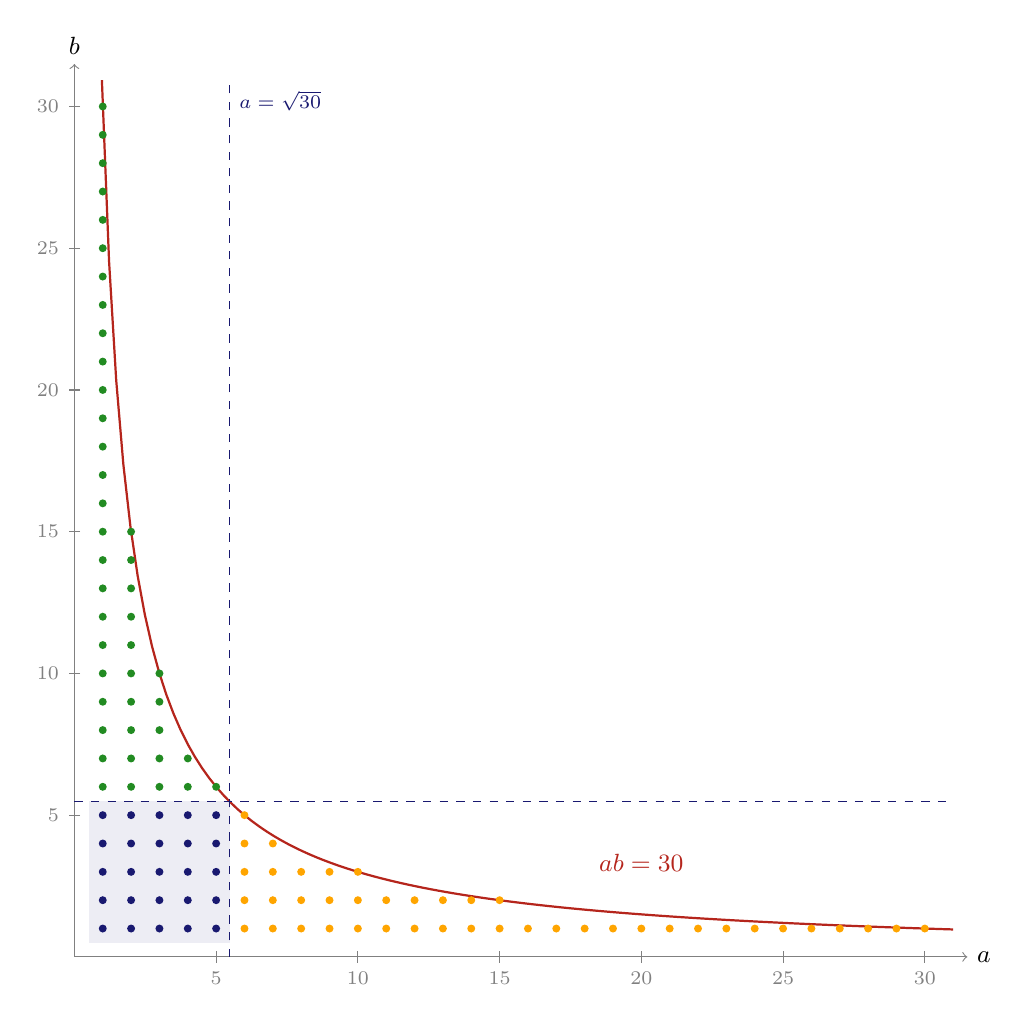
\begin{tikzpicture}[scale=0.36]
\fill[MidnightBlue!8] (0.5,0.5) rectangle (5.5,5.5);
\draw[->,gray] (0,0)--(31.5,0) node[right,black,font=\small] {$a$};
\draw[->,gray] (0,0)--(0,31.5) node[above,black,font=\small] {$b$};
\draw[gray] (5,0.2)--(5,-0.2) node[below,font=\scriptsize] {5};
\draw[gray] (0.2,5)--(-0.2,5) node[left,font=\scriptsize] {5};
\draw[gray] (10,0.2)--(10,-0.2) node[below,font=\scriptsize] {10};
\draw[gray] (0.2,10)--(-0.2,10) node[left,font=\scriptsize] {10};
\draw[gray] (15,0.2)--(15,-0.2) node[below,font=\scriptsize] {15};
\draw[gray] (0.2,15)--(-0.2,15) node[left,font=\scriptsize] {15};
\draw[gray] (20,0.2)--(20,-0.2) node[below,font=\scriptsize] {20};
\draw[gray] (0.2,20)--(-0.2,20) node[left,font=\scriptsize] {20};
\draw[gray] (25,0.2)--(25,-0.2) node[below,font=\scriptsize] {25};
\draw[gray] (0.2,25)--(-0.2,25) node[left,font=\scriptsize] {25};
\draw[gray] (30,0.2)--(30,-0.2) node[below,font=\scriptsize] {30};
\draw[gray] (0.2,30)--(-0.2,30) node[left,font=\scriptsize] {30};
\draw[BrickRed,thick,domain=0.97:31,samples=120] plot (\x,{30/\x});
\node[BrickRed,font=\small] at (20,3.3) {$ab=30$};
\draw[MidnightBlue,dashed] (5.47723,0)--(5.47723,31) (0,5.47723)--(31,5.47723);
\node[MidnightBlue,font=\scriptsize,above right] at (5.47723,29.5) {$a=\sqrt{30}$};
\fill[MidnightBlue] (1,1) circle (4pt);
\fill[MidnightBlue] (1,2) circle (4pt);
\fill[MidnightBlue] (1,3) circle (4pt);
\fill[MidnightBlue] (1,4) circle (4pt);
\fill[MidnightBlue] (1,5) circle (4pt);
\fill[ForestGreen] (1,6) circle (4pt);
\fill[ForestGreen] (1,7) circle (4pt);
\fill[ForestGreen] (1,8) circle (4pt);
\fill[ForestGreen] (1,9) circle (4pt);
\fill[ForestGreen] (1,10) circle (4pt);
\fill[ForestGreen] (1,11) circle (4pt);
\fill[ForestGreen] (1,12) circle (4pt);
\fill[ForestGreen] (1,13) circle (4pt);
\fill[ForestGreen] (1,14) circle (4pt);
\fill[ForestGreen] (1,15) circle (4pt);
\fill[ForestGreen] (1,16) circle (4pt);
\fill[ForestGreen] (1,17) circle (4pt);
\fill[ForestGreen] (1,18) circle (4pt);
\fill[ForestGreen] (1,19) circle (4pt);
\fill[ForestGreen] (1,20) circle (4pt);
\fill[ForestGreen] (1,21) circle (4pt);
\fill[ForestGreen] (1,22) circle (4pt);
\fill[ForestGreen] (1,23) circle (4pt);
\fill[ForestGreen] (1,24) circle (4pt);
\fill[ForestGreen] (1,25) circle (4pt);
\fill[ForestGreen] (1,26) circle (4pt);
\fill[ForestGreen] (1,27) circle (4pt);
\fill[ForestGreen] (1,28) circle (4pt);
\fill[ForestGreen] (1,29) circle (4pt);
\fill[ForestGreen] (1,30) circle (4pt);
\fill[MidnightBlue] (2,1) circle (4pt);
\fill[MidnightBlue] (2,2) circle (4pt);
\fill[MidnightBlue] (2,3) circle (4pt);
\fill[MidnightBlue] (2,4) circle (4pt);
\fill[MidnightBlue] (2,5) circle (4pt);
\fill[ForestGreen] (2,6) circle (4pt);
\fill[ForestGreen] (2,7) circle (4pt);
\fill[ForestGreen] (2,8) circle (4pt);
\fill[ForestGreen] (2,9) circle (4pt);
\fill[ForestGreen] (2,10) circle (4pt);
\fill[ForestGreen] (2,11) circle (4pt);
\fill[ForestGreen] (2,12) circle (4pt);
\fill[ForestGreen] (2,13) circle (4pt);
\fill[ForestGreen] (2,14) circle (4pt);
\fill[ForestGreen] (2,15) circle (4pt);
\fill[MidnightBlue] (3,1) circle (4pt);
\fill[MidnightBlue] (3,2) circle (4pt);
\fill[MidnightBlue] (3,3) circle (4pt);
\fill[MidnightBlue] (3,4) circle (4pt);
\fill[MidnightBlue] (3,5) circle (4pt);
\fill[ForestGreen] (3,6) circle (4pt);
\fill[ForestGreen] (3,7) circle (4pt);
\fill[ForestGreen] (3,8) circle (4pt);
\fill[ForestGreen] (3,9) circle (4pt);
\fill[ForestGreen] (3,10) circle (4pt);
\fill[MidnightBlue] (4,1) circle (4pt);
\fill[MidnightBlue] (4,2) circle (4pt);
\fill[MidnightBlue] (4,3) circle (4pt);
\fill[MidnightBlue] (4,4) circle (4pt);
\fill[MidnightBlue] (4,5) circle (4pt);
\fill[ForestGreen] (4,6) circle (4pt);
\fill[ForestGreen] (4,7) circle (4pt);
\fill[MidnightBlue] (5,1) circle (4pt);
\fill[MidnightBlue] (5,2) circle (4pt);
\fill[MidnightBlue] (5,3) circle (4pt);
\fill[MidnightBlue] (5,4) circle (4pt);
\fill[MidnightBlue] (5,5) circle (4pt);
\fill[ForestGreen] (5,6) circle (4pt);
\fill[Orange] (6,1) circle (4pt);
\fill[Orange] (6,2) circle (4pt);
\fill[Orange] (6,3) circle (4pt);
\fill[Orange] (6,4) circle (4pt);
\fill[Orange] (6,5) circle (4pt);
\fill[Orange] (7,1) circle (4pt);
\fill[Orange] (7,2) circle (4pt);
\fill[Orange] (7,3) circle (4pt);
\fill[Orange] (7,4) circle (4pt);
\fill[Orange] (8,1) circle (4pt);
\fill[Orange] (8,2) circle (4pt);
\fill[Orange] (8,3) circle (4pt);
\fill[Orange] (9,1) circle (4pt);
\fill[Orange] (9,2) circle (4pt);
\fill[Orange] (9,3) circle (4pt);
\fill[Orange] (10,1) circle (4pt);
\fill[Orange] (10,2) circle (4pt);
\fill[Orange] (10,3) circle (4pt);
\fill[Orange] (11,1) circle (4pt);
\fill[Orange] (11,2) circle (4pt);
\fill[Orange] (12,1) circle (4pt);
\fill[Orange] (12,2) circle (4pt);
\fill[Orange] (13,1) circle (4pt);
\fill[Orange] (13,2) circle (4pt);
\fill[Orange] (14,1) circle (4pt);
\fill[Orange] (14,2) circle (4pt);
\fill[Orange] (15,1) circle (4pt);
\fill[Orange] (15,2) circle (4pt);
\fill[Orange] (16,1) circle (4pt);
\fill[Orange] (17,1) circle (4pt);
\fill[Orange] (18,1) circle (4pt);
\fill[Orange] (19,1) circle (4pt);
\fill[Orange] (20,1) circle (4pt);
\fill[Orange] (21,1) circle (4pt);
\fill[Orange] (22,1) circle (4pt);
\fill[Orange] (23,1) circle (4pt);
\fill[Orange] (24,1) circle (4pt);
\fill[Orange] (25,1) circle (4pt);
\fill[Orange] (26,1) circle (4pt);
\fill[Orange] (27,1) circle (4pt);
\fill[Orange] (28,1) circle (4pt);
\fill[Orange] (29,1) circle (4pt);
\fill[Orange] (30,1) circle (4pt);
\end{tikzpicture}
